\documentclass[]{article}
\usepackage{graphicx}
\usepackage{hyperref}
\usepackage{float}

%opening
\title{Assignment 2 CDA}
\author{Tim van Rossum, 4246306\\
	Michiel Doesburg, 4343875}

\begin{document}

\maketitle
\section{Familiarization with the data}
The dataset contains a total of 44 signals, with some being static values, other being sinusoid signals, and others being partially discrete (as in, they can rise or drop at certain points). L-signals tend to be more sinusoidal, F-signals tend to be "partially discrete", and S-signals are all binary signals.

All the signals together seem to have little correlation. Some combinations of signals are reasonably correlated: e.g. L\_T3 and P\_J302 have a 0.42 correlation coefficient. Moreover, the signal P\_J302 in figure~\ref{correlation} looks cyclic. A cyclic signal like this is much easier to predict than a `random' signal, since there is a rough base model that it adheres to. This signal's values are within a clear band at about 2-6 on the Y-axis. In such a case it is very easy to come up with a basic anomaly detection technique: if the signal moves outside this band this would be a clear sign of an anomaly. Plotting the mean error we saw for the ARMA prediction on signal L\_T1, we saw that there were only 2 cases were the error was greater than three times the standard deviation. 

\begin{figure}[H]
\begin{minipage}{.5\textwidth}
  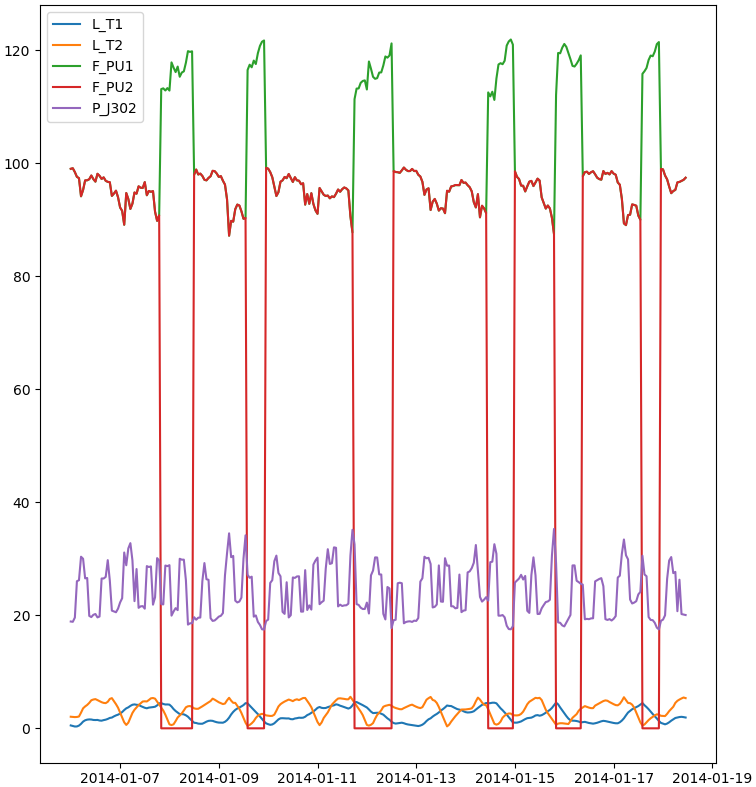
\includegraphics[width=0.8\linewidth, keepaspectratio]{./visuallizations/signals.png}
  \caption{Visualization of some signals. The red and greens signals are partially discrete.}
  \label{signals}
\end{minipage} %
\begin{minipage}{.5\textwidth}
  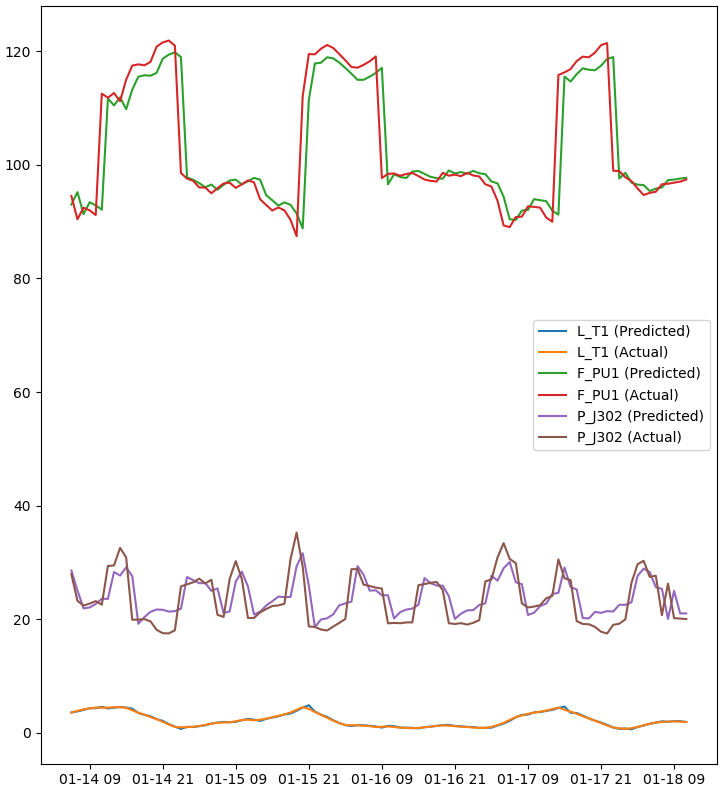
\includegraphics[width=0.8\linewidth, keepaspectratio]{./visuallizations/predictions.png}
   \caption{ARMA predictions on some signals. The predictions work better on signals.with less variance}
  \label{predictions}
\end{minipage}
\begin{minipage}{.5\textwidth}
  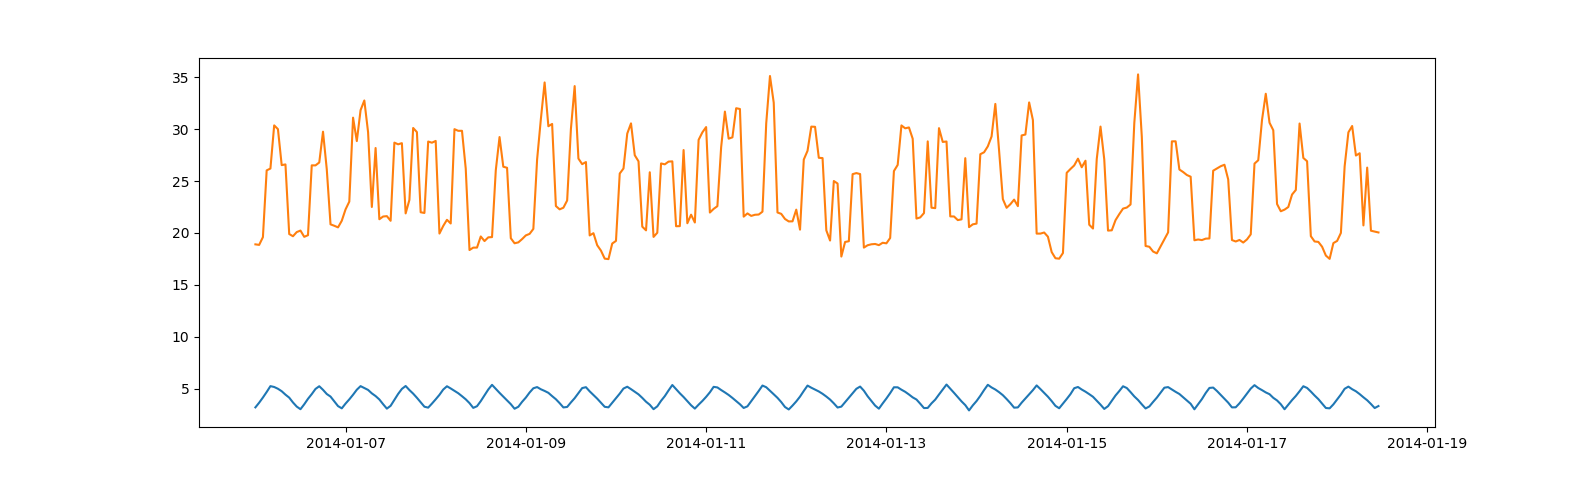
\includegraphics[width=2\linewidth, height=4cm]{./visuallizations/correlated_signals.png}.
  \label{correlation}
  \caption{Signals L\_T3 and P\_J302. The peaks are roughly aligned.}
\end{minipage}%
\end{figure}

\section{ARMA}
\section{Discrete models}
\section{PCA}
\section{Comparison} 

\end{document}
